\documentclass[12pt, twoside]{article}
\documentclass[12pt, twoside]{article}
\usepackage[letterpaper, margin=1in, headsep=0.2in]{geometry}
\setlength{\headheight}{0.6in}
%\usepackage[english]{babel}
\usepackage[utf8]{inputenc}
\usepackage{microtype}
\usepackage{amsmath}
\usepackage{amssymb}
%\usepackage{amsfonts}
\usepackage{siunitx} %units in math. eg 20\milli\meter
\usepackage{yhmath} % for arcs, overparenth command
\usepackage{tikz} %graphics
\usetikzlibrary{quotes, angles}
\usepackage{graphicx} %consider setting \graphicspath{{images/}}
\usepackage{parskip} %no paragraph indent
\usepackage{enumitem}
\usepackage{multicol}
\usepackage{venndiagram}

\usepackage{fancyhdr}
\pagestyle{fancy}
\fancyhf{}
\renewcommand{\headrulewidth}{0pt} % disable the underline of the header
\raggedbottom
\hfuzz=2mm %suppresses overfull box warnings

\usepackage{hyperref}
\usepackage{float}

\fancyhead[LE]{\thepage}
\fancyhead[RO]{\thepage \\ First and last name: \hspace{2.5cm} \,\\ Section: \hspace{2.5cm} \,}
\fancyhead[LO]{BECA / Dr. Huson / Regents Prep: Graphs\\* 18 November 2024}

\begin{document}

\subsubsection*{3.4 Do Now: Graphing quadratic systems}
\begin{enumerate}
  \item One equation of a system is graphed. 
\begin{enumerate}
    \item Graph the second equation, labeling the intersections as ordered pairs.
    \item Find the value of the leading coefficient $a$ of the quadratic equation.
\end{enumerate}
    \begin{multicols}{2}
      \hspace{1cm} $y = ax^2 + 3x - 7$ \\
      \columnbreak
      $3x - y = -3$
      \end{multicols}
       \vspace{3cm}
  
    \begin{center}
    \begin{tikzpicture}[scale=.635]
      \draw [help lines] (-10,-10) grid (10,10);
      \draw [thick, ->] (-10.2,0) -- (10.4,0) node [below right] {$x$};
      \draw [thick, ->] (0,-10.2)--(0,10.4) node [left] {$y$};
      \draw[thick, <->,smooth, domain=-3.3:2.1] plot (\x, {2.5*(\x)^2 + 3*\x - 7});
    \end{tikzpicture}
    \end{center}

\newpage
\item Identify the expressions that are equal to $\displaystyle \frac{4^2}{4^4}$
  \begin{multicols}{2}
  \begin{enumerate}
      \item $\displaystyle \frac{1}{4^2}$
      \item $4^{-2}$
      \item $\frac{1}{16}$
      \item $4^6$
      \item $4^{2}$
      \item $0.0625$
  \end{enumerate}
  \end{multicols}

\item Identify the expressions that are equal to $\displaystyle 4^{-2}$
  \begin{multicols}{2}
    \begin{enumerate}
        \item $\displaystyle \frac{1}{4^2}$
        \item $0.0625$
        \item $\displaystyle \frac{1}{16}$
        \item $4.25$
        \item $2$
        \item $\sqrt{4}$
    \end{enumerate}
    \end{multicols}
    \item Identify the expressions that are equal to $\displaystyle 27^{\frac{1}{3}}$
      \begin{multicols}{2}
      \begin{enumerate}
          \item $3$
          \item $9$
          \item $\sqrt[3]{27}$
          \item $27.33$
          \item $1.5$
          \item $81$
      \end{enumerate}
      \end{multicols}

    \item The graph of the function $f(x) = x^3 - 3x^2 - 4x + 12$ is shown. Write the function in factored form. 
    \begin{flushright}
    \begin{tikzpicture}[xscale=1, yscale=0.3]
        \draw [thick, ->] (-4.2,0) -- (5,0) node [above] {$x$};
        \draw [thick, ->] (0,-8.2)--(0,12) node [right] {$y$};
        \foreach \x in {-3,...,4} \draw (\x cm,12pt) -- (\x cm,-12pt) node[below] {$\x$};
        \foreach \y in {12*0.7} \draw (3pt,\y cm) -- (-3pt,\y cm) node[left] {12};
        \draw [thick, <->,smooth,samples=20,domain=-2.6:4.2] plot(\x,{0.7*(\x-2)*(\x-3)*(\x+2)});
    \end{tikzpicture}
    \end{flushright}

\end{enumerate}
\end{document}